\documentclass[../main]{subfile}
\graphicspath{\subfix{../images}}
\begin{document}

Fast R-CNN完成微调后,检测除了要运行一个前向传播还有一些其他步骤(假设物体候选已经被预先计算好)。网络将一张图片(或者一个图片金字塔,编码为一个图片列表)以及包含$R$个将要打分的物体候选作为输入。在测试时,虽然我们将会考虑$R$更大($\approx 45\text{k}$)的情形,但是$R$通常是2000。\textcolor{violet}{当使用图片金字塔时,每个RoI都会分配给尺寸这样缩放后的RoI在区域中与$224^2$像素最接近。}

对于每一个测试RoI $r$,前向传播输出一个类别后验概率分布$p$以及一系列与$r$相关的预测边界框偏移($K$类中的每一个类得到它自己的调整后的边界框预测)。我们使用估计的概率$\text{Pr}(\text{class}=k|r)\triangleq p_k$对每一个物体类别$k$为$r$赋值一个检测置信度。我们接下来独立为每一个类进行非最大抑制,其中使用的算法和设置与R-CNN\cite{rcnn}相同。

\subsection{为了更快的检测进行SVD裁剪}

\begin{figure}[hb]
    \centering
    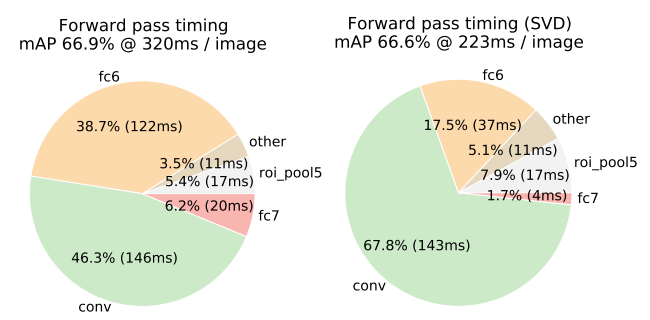
\includegraphics[width=.9\textwidth]{fig2.png}
    \caption{SVD裁剪前后的时间情况。在SVD之前,全连接层fc6和fc7占了45\%的时间}
    \label{fig:img2}
\end{figure}

对于整张图片的分类,与卷积层花费的时间相比,全连接层花费的时间是少的。与之相反的是,由于要处理的RoI数量很大所以几乎一半的前向传播时间是花费在全连接层上的(见图\ref{fig:img2})。通过使用裁剪SVD来将大的全连接层压缩可以轻易实现加速。

在这个技术中,被参数化为$u \times v$系数矩阵$W$的一层可以使用SVD被近似分解为:
\begin{equation}
    W \approx U \Sigma_tV^\top
\end{equation}
在这个分解中,$U$是一个有$W$的前$t$个左特征值向量组成的形状为$u \times t$的矩阵,$\sum_t$是包含$W$的前$t$大的特征值的$t\times t$的对角阵。裁剪SVD将参数量从$uv$变为了$t(u+v)$,当$t$远小于$\min(u, v)$时效果是显著的。为了压缩一个网络,一个对应$W$的全连接层被替换为两个全连接层,二者之间没有非线性。其中的第一层使用系数矩阵$\Sigma_t V^\top$(没有偏差),第二层使用$U$(使用与$W$关联的原始偏差)。当RoI数量很大时,这个简单的压缩方法提高了速度。
\end{document}